

\documentclass[12pt]{article}

% Paquete para gráficos
\usepackage{graphics}
\usepackage{graphicx}
\usepackage{caption}
\usepackage[spanish]{babel}
\usepackage{float}
\usepackage{hyperref}
\usepackage{booktabs}
\usepackage{multirow}
\usepackage{siunitx}
\sisetup{
  round-mode          = places, % Redondeo
  round-precision     = 2, %  solo 2 decimales
}

\author{Estudiante 1, Estudiante 2, y Estudiante 3}
\date{\today}
\title{Proyecto de CA-0203}

\begin{document}

\maketitle

% Tabla de contenidos
\newpage
\tableofcontents

\newpage

%Seccion 2: tipo de cambio forward
\section{Análisis del Contrato Forward de Tipo de Cambio y Estrategia para Mitigación de Riesgo Cambiario}

\subsection*{Determinación del precio del contrato forward}

Para determinar el precio en colones del contrato forward, es fundamental replicar los flujos futuros del contrato en el momento \( T \) mediante una estrategia de inversión equivalente. Este enfoque se basa en el principio de \textbf{ausencia de arbitraje}, que establece que dos activos con flujos de efectivo idénticos deben tener el mismo precio. De lo contrario, sería posible obtener ganancias sin riesgo mediante arbitraje al comprar el activo más barato y vender el más caro.

La estrategia para replicar los flujos del contrato forward sería la siguiente:

\begin{enumerate}
    \item \textbf{Venta de bonos cero cupón en colones}: Se venden bonos cero cupón por un monto nominal de \( K \) colones en el momento \( t \). Esto garantiza que en el momento \( T \) se tendrá la obligación de pagar \( K \) colones.
    \item \textbf{Compra de un bono cero cupón en dólares}: Se adquiere un bono cero cupón de la Reserva Federal de Estados Unidos (FED) en el momento \( t \), con un valor de compra equivalente a \( E_t \cdot P_{\text{\$}}(t, T) \) colones, donde \( E_t \) es el tipo de cambio actual y \( P_{\text{\$}}(t, T) \) es el precio del bono. Este bono garantizará la entrega de 1 dólar en \( T \), que al venderse se convierte en \( E_T \) colones en ese momento.
\end{enumerate}

El costo de esta estrategia en \( t \) será:
\[
kP_{\text{₡}}(t, T) - E_t P_{\text{\$}}(t, T),
\]
donde \( P_{\text{₡}}(t, T) \) es el precio actual de un bono cero cupón en colones. Este valor representa el precio justo del contrato forward, ya que replica perfectamente los flujos futuros.

\subsection*{Proyección del tipo de cambio futuro}

Para anticipar el comportamiento del tipo de cambio y calcular el forward, es necesario identificar el monto \( K \) que hace que el valor del contrato en \( t \) sea cero. Este valor se obtiene como:
\[
k = \frac{E_t \cdot P_{\text{\$}}(t, T)}{P_{\text{₡}}(t, T)},
\]
lo que indica el tipo de cambio forward.

Esta fórmula implica que el tipo de cambio forward es el mejor estimador del tipo de cambio esperado \( E_T \) bajo el principio de ausencia de arbitraje. La lógica detrás de esto es que, si ambas partes del contrato se ponen de acuerdo en que intercambiar \( E_T \) por $\frac{E_t \cdot P_{\text{\$}}(t, T)}{P_{\text{₡}}(t, T)}$ en \( T \) hace que el precio del contrato sea 0, entonces eso significa que a ambas partes les es indiferente participar o no en el contrato; en otras palabras, para la empresa ABC sería lo mismo asegurar un intercambio de \( E_T \) por $\frac{E_t \cdot P_{\text{\$}}(t, T)}{P_{\text{₡}}(t, T)}$ a través de un contrato forward de tipo de cambio o simplemente esperar a pagar el \( E_T \) que determine el mercado en el futuro. 

Por tanto, para la planificación presupuestaria de la empresa, el valor de $\frac{E_t \cdot P_{\text{\$}}(t, T)}{P_{\text{₡}}(t, T)}$ debe ser tomado como referencia para prever el costo de los insumos en dólares al final de cada mes durante los próximos cinco años.
\begin{figure}[H]
    \centering
    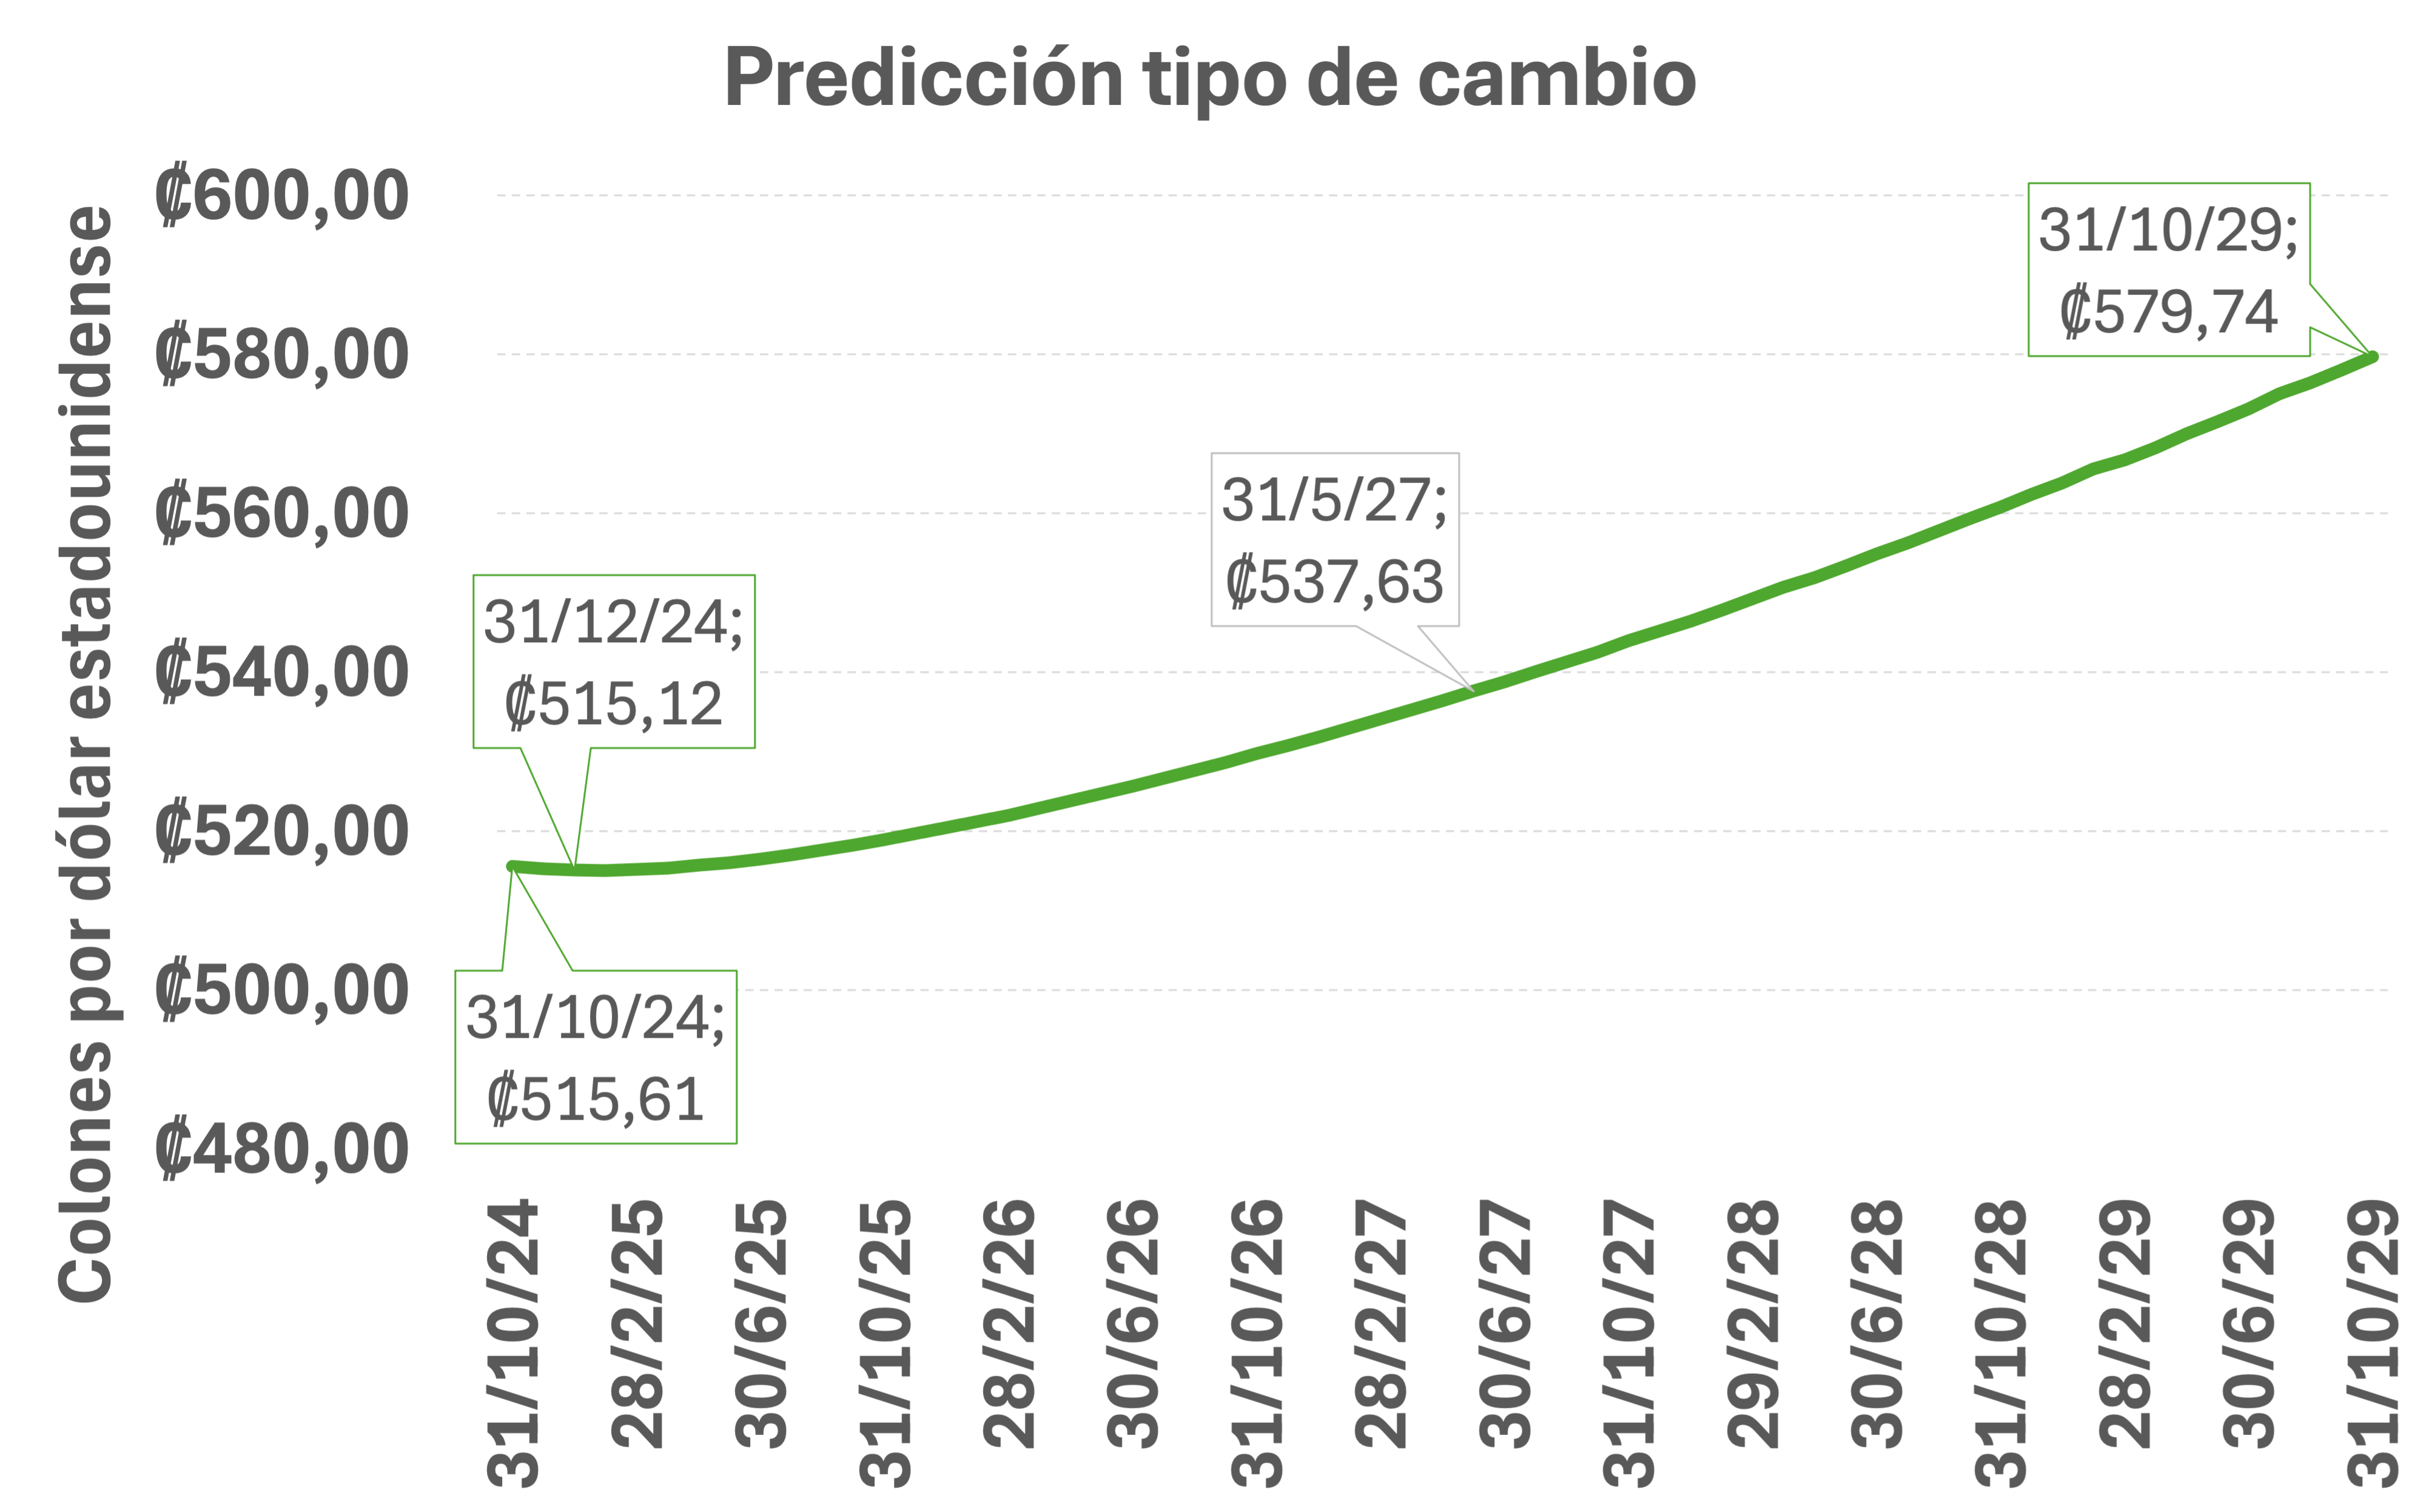
\includegraphics[width=1\linewidth]{grafico_tipo_de_cambio.png}
    \caption{Proyección del tipo de cambio \( E_T \) en los próximos 5 años}
    \label{fig:enter-label}
\end{figure}

\subsection*{Demostración de arbitraje con un tipo de cambio futuro de ₡500 por dólar al 31/12/2024}

En el escenario hipotético donde el tipo de cambio efectivo al 31 de diciembre de 2024 sea \( E_T = 500 \, \text{colones/dólar} \), se observa que este valor sería menor al tipo de cambio forward calculado como:
\[
k = \frac{E_t \cdot P_{\text{\$}}(t, T)}{P_{\text{₡}}(t, T)} = 515,12
\]
Esto abriría la posibilidad de arbitraje:

\begin{itemize}
    \item Un arbitrajista podría vender un contrato forward de tipo de cambio, comprometiéndose a entregar \( E_T \) colones a cambio de \( k \).
    \item En este caso, se asegura una ganancia igual a:
    \[
    k - E_T = \frac{E_t \cdot P_{\text{\$}}(t, T)}{P_{\text{₡}}(t, T)} - 500 = 15,12
    \]
    colones por dólar.
\end{itemize}

Dado que el contrato forward se negocia de forma que su precio inicial sea cero, no habría costos presentes, lo que garantiza que cualquier diferencia futura positiva entre \( k \) y \( E_T \) represente una ganancia asegurada para el arbitrajista.

\subsection*{Conclusión y recomendación}

La implementación de un contrato forward de tipo de cambio representa una herramienta eficaz para mitigar el riesgo cambiario al fijar el tipo de cambio de las transacciones futuras. Basándonos en las proyecciones forward, se recomienda considerar el nivel \( k \) como referencia clave para definir los presupuestos y asegurar la estabilidad financiera de la empresa frente a la volatilidad cambiaria.


% Finalizamos el documento
\end{document}
